% what does it mean? Interpret the patterns observed within the data. Link back to a broader discussion.

Shipping is a major user of the ocean, but little is known about its distribution and effects. Here I built the first validated and global models of ship movement, to better enable us to manage the ocean effectively. The shipping companies acknowledge the importance of managing the ocean holistically, but lack the scientific knowledge and tools to do so effectively. By incorporating ecological information alongside logistical efficiencies, it should be possible to improve the system robustness.

Marine protected areas (MPAs) have been shown to be effective~\citep{halpern2002marine}, but the multidimensional nature of ocean use is pointing toward dynamic MPAs,\citep{Boersma1999} % Looks good. May be worth looking at things like Boersma and Parrish, 1999 "Limiting Abuse: marine protected areas, a limited solution" to get a sense of how cumulative risk can still mean that low probability events can be worth paying attention to in this space. But definitely: improved regulation, addition of MPAs, introduction of AIS have all helped limit exposure to this risk.

 which may rely on providing users, such as ship operators, with real-time information about the state of the environment. Marine spatial planning is proving a promising avenue for brining stakeholders together~\citep{merrifield2012marinemap}. This new form of planning has greater data requirements, which in the ocean can be simplified down to three major areas of use: fisheries management, transportation management, and energy management. Transportation in the ocean is the least studied of the three, and here we have shown how volunteered geographic information methods, along with volunteered observations, can provide us a way to tackle the data-poor problem.

% XXX FORMAT THIS AROUND THE TALK SLIDES

% XXX REMOVE THIS? Don't really need it, was really just filler till I had my act together. Explain, IN WORDS, why this matters and integrate those changes into the body of the thesis.
%\begin{figure}[h!]
%  \centering
%    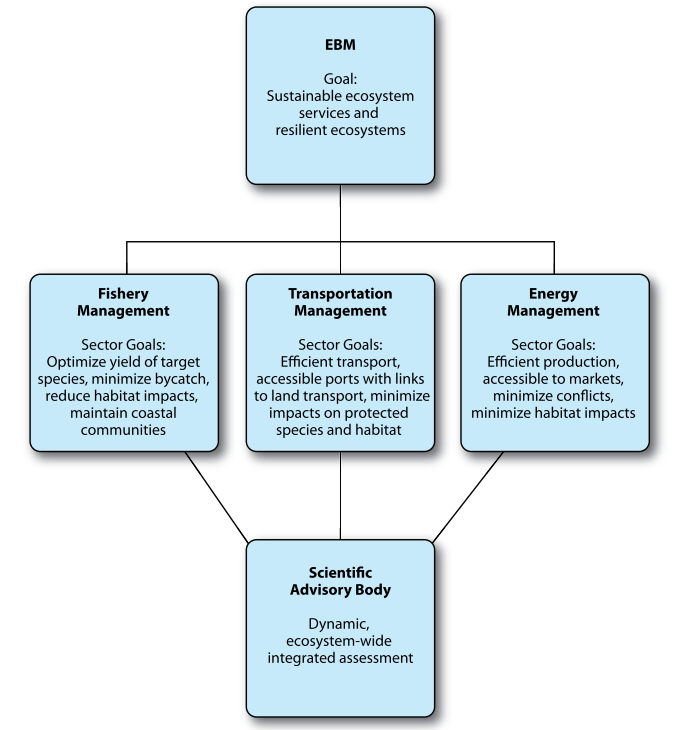
\includegraphics[width=90mm]{figures/lubechenco-diagram.png}
%  \caption[Framing Ecosystem-based management goals]{Framing ecosystem-based management goals, as in \cite{Lubchenco2010}; original from \citep{McLeod2009}}
%  \label{fig:framing}
%\end{figure}
% XXX INCLUDE THE GOALS IN TEXT, fisheries management, transportation, energy production.

% XXX XXX XXX EXTENT OF DETAILED DATA
 This paper contributes rich data predominantly within 100km of shores, where most human and biological users of the ocean persist, and building our knowledge of these areas is particularly valuable. Ship traffic is most dense, regulated, and complex within the exclusive economic zones of nations, and it is useful property that this data are dense within these areas.
% XXX oliver: It might be worth expanding on "where most human and biological users of the ocean persist".  It's worth emphasizing that most of the stuff we care about occurs in this region, which is also where ship traffic is the most common, the hardest to predict (lots of ships of all sorts, lots of destinations), and the most regulated (shipping lanes).
% XXX XXX

% XXX XXX REGULATION AS IMPORTANT SECTION XXX XXX

The primary extractive use of the ocean is the fishing, where our understanding has been advanced by intensive investments to study its effects. % XXX citation for this? its clear from spending, but quantify it.
Many fisheries are now managed systems~\citep{worm2009rebuilding}, as unmanaged fish stocks have repeatedly collapsed~\citep{costello2012status}. % clearly disagreement in the Worm / Jackson / Halpern vs. Hilborn camps, use their joint papers as an end-run around this.

Similar management and regulation is noticeably absent from the shipping industry.
% XXX oliver: JUMPED FROM FISHING TO INSURANCE, DO I ACTUALLY DO ANYTHING WITH THIS STUFF? Not really. ?bro
  Shipping is regulated by the International Maritime Organization (IMO), a branch of the United Nations which enforces industry rules and standards. However, the transnational nature of the industry has led to low enforcement rates. As is common in consensus-based international bodies~\citep{cogan2009representation}, the IMO is slow to respond to problems of the day. 
  % XXX have to cite both of these statements if this is gonna stick. INSTEAD: say that they are a CONSENSUS based organization which requires ratification of many international bodies, by its nature a time consuming process. 
  For example, while acknowledging that 20\% reductions in greenhouse gasses can be accomplished in this decade, without additional costs to operators \citep{imo2009}, it has not implemented new emissions rules.  In light of the regulatory environment, alternatives, such as tying ship insurance rates to ecologically important areas of the ocean, may be preferable.
 % an example article on IMO problems: http://articles.cnn.com/2012-07-04/world/world_europe_costa-concordia_1_concordia-disaster-cruise-industry-cruise-ship-disaster/3?_s=PM:EUROPE
 % http://ban.org/ban_news/2006/060316_imo_treaty.html
 % http://www.sourcewatch.org/index.php?title=International_Maritime_Organization#Criticisms_of_the_IMO

%   + other parts of the ocean environment coming into regulation, particularly fishing
%   + Regulation of shipping rudimentary
%    * wild west in terms of control; do regulate emissions in specific places but international agreements minimal (what's IMO got on the table)
%    * part of the problem is that shipping is extremely international, more so than fishing
%    * primary regulation is at ports, otherwise just GPS units and a hope that no one crashes


% XXX XXX XXX


% XXX XXX Oliver: By now, I've lost track of why I should care about transportation networks.  How do transportation networks affect the things you've discussed in the previous section?  Is there something inherent in their nature or structure that's particularly relevant?  If you're just pointing out that there's not a lot of useful data available, is it worth it's own section?
\subsection{Transportation Networks}
One approach to managing a complex system like shipping is to study its network representation.  Transportation networks with geographically-fixed edges and nodes, such as road and rail, form the basis of transportation geography \citep{Rodrigue2009}. Unlike these networks, shipping exists in between the extremes of a fixed network % XXX DEFINE, Newman 2010?
 and two dimensional Brownian bridges, as vessels must transport both goods and passengers to specific locations (primarily ports) but are free in choosing movement between destinations, except in near shore areas regulated by shipping lanes. Air transportation shares network similarities, but strong regulation has led to predetermined flight paths, with deviations generally limited to emergencies or extreme weather. % XXX need a ref here. how does the FAA and the relevant international body regulate movement? XXX XXX find something, in transportation geography book? where?

Because of inherent risks in air transportation, detailed, well-vetted information on flight paths is provided by government agencies \citep{guimera2005worldwide}, simplifying modeling. Ship movements have no equivalent top-down data collection effort, and while organizations such as the US Coast Guard have made efforts, the system remains rudimentary. Most information is provided via private contracts, through organisations such as Lloyd's of London, who have been recording information on shipping since 1774 \citep{Lloyd'sRegister-FairplayLtd.2010}. As a result, limited public data are available on the shipping trade, despite being identified by the Federal Geographic Data Committee~\citep{FGDC} as a key transportation component to the national spatial data infrastructure \citep{CurrierInPress}.

% XXX where are you going with this?
Transportation networks play an important economic role \citep{canning1993effects}. Because this role, information on shipping is valuable, leading to a cottage industry of information sales and limiting its public availability. Here, we look at using geographically-volunteered information to infer the movement patterns which in part define the shipping network.

% TALK ABOUT OTHER MODES OF TRANSPORTATION; [this gives you a way to tame it, its reasonable to assume that it'll map to one of these models]

% - shipping has big economic benefit, but costs are externalized
% - there are good actors in shipping who want to do the right thing, but don't have the tools to do it [cites, +Maersk lady]
% - only scientific community can do this
% - can only do msp by bringing stakeholders together
% - VGI methods provide good way of handling messy data as we try to move it toward 'reality'
% - coupling these approaches with real-time efforts has potential to shift dynamic.

% XXX XXX Goodchild: there's an opportunity to attach probabilities to individual points based on other points in the track.

% XXX BONUS STUFF ON BALLAST:
While most species don't meet the criteria for establishing ecological viability in the system, ballast exchange does introduce ecological coupling between otherwise disconnected systems. This interchange can cause localized problems to become global ones, particularly for viruses and bateria, which have human health consequences beyond ecosystem function. 

The ballast water situation in the US is generally better because of the higher compliance with ballast exchange points, and stricter enforcement, including some preliminary isotopic work. Higher cost structures for shipping industry means pushback but their absorbed costs still much smaller than the economic impacts of invasives.

% XXX BONUS STUFF ON LINKAGES TO OTHER FIELDS
Other domains, such as ecology and economics, are coming to terms with the fact that their historical approaches to keeping simple models (and by extension, limiting model scope to their domain) ignores important spatial context which naturally arises at the unit of analysis \citep{tilman1997,krugman1991geography}.


